\documentclass{article}
\usepackage[utf8]{inputenc}
\usepackage[top=1in, bottom=1in, left=1in, right=1in]{geometry}
% \usepackage{indentfirst}
\usepackage{amsmath}
\usepackage{amssymb}
\usepackage{graphicx}
    \DeclareGraphicsExtensions{.png, .jpeg}
\usepackage{caption}

% custom macros
\newcommand*{\doublebar}[1]{\overline{\overline{#1}}}
\newcommand*{\unknown}[0]{\;?\;}
\DeclareMathOperator*{\argmax}{argmax}


% main document
\title{MATH 786: Cooperative Game Theory \\ HW02}
\author{Terence Henriod}
\date{\today}

\begin{document}

\maketitle

\begin{abstract}
Convex Games, Balanced Games, Shapley-Bondareva Theorem, Market Games.
\end{abstract}


\newpage
\begin{enumerate}
\item Give an example of a 3-player balanced game which is not convex. \\

\textit{Solution}: \\
Let $G = (N, V)$ where 
\[
N = \{1, 2, 3\}
\]
and
\[
    V(S) = \begin{cases}
        |S|  & \text{ if } |S| > 1 \\
        0    & \text{ otherwise}
    \end{cases}
\]

Recall that for a game to be balanced, then
\[ \sum_{S \in T}{\delta_{S}V(S)} \le V(N) \qquad \circledast \]
must be true for all balanced families, $T$, of $G$.
The following table displays all of the minimal balanced families of $G$. Non-minimal balanced families are not considered because they are trivially balanced using a weight of 0 for the ``extraneous" coalitions and will meet the $\circledast$ criterion just as the minimal balanced families.

\begin{tabular}{| l | c | l |}
    \hline
    $T$                                                          &  $\{\delta_{S}\}$                         &  
    $\circledast$ Check \\
    \hline\hline
    $\{\overline{1}, \overline{2}, \overline{3}\}$               &  $1, 1, 1$                                &  
    $1 * 0 + 1 * 0 + 1 * 0 = 0 \le 3 \implies \text{OK}$ \\
    \hline
    $\{\overline{1, 2}\,, \overline{3}\}$                        &  $1, 1$                                   & 
    $1 * 2 + 1 * 0 = 2 \le 3 \implies \text{OK}$ \\
    \hline
    $\{\overline{1, 3}\,, \overline{2}\}$                        &  $1, 1$                                   & 
    $1 * 2 + 1 * 0 = 2 \le 3 \implies \text{OK}$ \\
    \hline
    $\{\overline{2, 3}\,, \overline{1}\}$                        &  $1, 1$                                   & 
    $1 * 2 + 1 * 0 = 2 \le 3 \implies \text{OK}$ \\
    \hline
    $\{\overline{1, 2, 3}\}$                                     &  $1$                                      & 
    $1 * 3 = 3 \le 3 \implies \text{OK}$ \\
    \hline
    $\{\overline{1, 2}\,, \overline{1, 3}\,, \overline{2, 3}\}$  &  $\frac{1}{2}, \frac{1}{2}, \frac{1}{2}$  & 
    $\frac{1}{2} * 2 + \frac{1}{2} * 2 + \frac{1}{2} * 2 = 3 \le 3 \implies \text{OK}$ \\
    \hline
\end{tabular} \\\\
$G$ is balanced. \\
To show that a game is not convex, then
\[ V(S_{1}) + V(S_{2}) > V(S_{1} \cup S_{2}) + V(S_{1} \cap S_{2}) \]
must be true for some pair $S_{1}$, $S_{2}$ in $2^{N}$. \\

Let $S_{1} = \overline{1, 2}$ and  $S_{2} = \overline{2, 3}$. Then we have:
\begin{align*}
V(\overline{1, 2}) + V(\overline{2, 3})  &>  V(\overline{1, 2, 3}) + V(\overline{2}) \\
2                  + 2                   &>  3                     + 0 \\
4                                        &>  3 \\ 
\end{align*}
Which is true. \\
Thus, $G$ is balanced and non-convex.

%
% \hfill\newline
\newpage
\item Recall the glove game from Problem Set \#1. We showed that this game had a nonempty core by exhibiting a core vector for any value of $m$ and $p$. [$m$ and $p$ were the numbers of left-hand and right-hand gloves in the game.] Now prove the core is nonempty again, this time by using the Shapley-Bondareva theorem. HINTS: A) You may assume without loss of generality that $m \le p$. B) For each $S_{i}$ in your arbitrary balanced family, define $\tilde{S_{i}}$ as a subset of $S_{i}$ for which a) $\tilde{S_{i}}$ contains equal numbers of left- and right-hand glove players; b) $V(\tilde{S_{i}}) = V(S_{i})$. \\

\textit{Solution}: \\
If the glove game has a non-empty core, than any arbitrary balanced family will satisfy:
\[\sum_{S_{i}}{\delta_{S_{i}} V(S_{i})} \le V(N)\]

So we have:
\begin{align*}
\sum_{S_{i} \in T}{\delta_{S_{i}} V(S_{i})}                                          &\le  V(N)  &   \\
\sum_{S_{i} \in T}{\delta_{S_{i}} V(\tilde{S_{i}})}                                  &\le  V(N)  &  \text{by the assumption in the hints} \\
\sum_{S_{i} \in T}{\delta_{S_{i}} * 5 * |\tilde{S_{i}} \cap M|}                      &\le  V(N)  &  M \text{ is the set of left-hand glove holding players} \\
\sum_{S_{i} \in T}{\delta_{S_{i}} * 5 * \sum_{j \in M}{|\tilde{S_{i}} \cap \{j\}|}}  &\le  V(N)  &   \\
5 * \sum_{j \in M}{\sum_{S_{i} \in T}{\delta_{S_{i}} |\tilde{S_{i}} \cap \{j\}|}}    &\le  V(N)  &   \\
5 * \sum_{j \in M}{\sum_{S_{i} \in T}{\delta_{S_{i}} |S_{i} \cap \{j\}|}}            &\le  V(N)  &  \text{because } |\tilde{S_{i}} \cap \{j\}| \le |S_{i} \cap \{j\}| \\
5 * \sum_{j \in M}{(1)}                                                              &\le  V(N)  &  \text{by definition of a balanced game} \\
5m                                                                                   &\le  V(N)  &   \\
5m                                                                                   &\le  5m    &   \\
\end{align*}

The idea: because of the balancing weights, each value $V(S)$ is ``scaled down" so that they will only sum to the value of the grand coalition, at most.

%
\hfill\newline
\item Determine if the following game has a nonempty core. If the core is nonempty, state a core vector; if not, present an argument using the Shapley-Bondareva Theorem.
$$N = \{1, 2, 3, 4\}$$
$$V(N) = 10$$
$$V(\overline{1, 4}) = V(\overline{1, 2, 4}) = V(\overline{1, 3, 4}) = 8$$
$$V(\overline{1, 2, 3}) = V(\overline{2, 3, 4}) = 7$$
$$V(S) = 0 \; \text{for all other coalitions} \; S$$

\textit{Solution}: \\
The game $G$ has an empty core. \\

The Shapley-Bondareva Theorem states that a game's core must be non-empty if that game is balanced; that is if:
\[ \sum_{S \in 2^{N}, \, S \neq \emptyset}{\delta_S V(S)} \le V(N) \]
for every balanced family $T$, where:
\[ \sum_{S \in 2^{N} \, : \, i \in S}{\delta_{S}} = 1, \; 0 \le \delta_{S} \le 1 \]

Consider the balanced family $T = \{\overline{1, 4},\; \overline{1, 2, 3},\; \overline{2, 3, 4}\}$. $T$ can be balanced with all weights $\delta_{S} = \frac{1}{2}$. Using the Shapley-Bondareva criterion, we have:
\begin{align*}
\frac{1}{2}V(\overline{1, 4}) + \frac{1}{2}V(\overline{1, 2, 3}) + \frac{1}{2}V(\overline{2, 3, 4})  &\le      V(\overline{1, 2, 3, 4}) \\
\frac{1}{2}(8)                + \frac{1}{2}(7)                   + \frac{1}{2}(7)                    &\le      (10) \\
\frac{8}{2}                   + \frac{7}{2}                      + \frac{7}{2}                       &\le      10   \\
\frac{22}{2}                                                                                         &    \le  10   \\
11                                                                                                   &\not\le  10   \\
\end{align*}
Since $T$ violates the condition, the core of $G$ must be empty.

%
\hfill\newline
\item Are all convex games market games? Give an argument or a counterexample. \\

\textit{Solution}: \\
Yes, all convex games are market games.

When we talk about convex games, by definition, all sub-games of a convex game are also convex. If a game is convex that means that it has a non-empty core. Having a non-empty core is equivalent to being a balanced game. Thus, all sub-games of a convex game are balanced. Since all sub-games of a convex game are balanced, the original convex game is totally balanced. All totally balanced games are market games. Thus, all convex games are market games.

%
\hfill\newline
\item Suppose given a market game in which $n = 3$ and $m = 2$. The initial endowments are $a^{1} = (1, 0)$, $a^{2} = (0, 3)$, and $a^{3} = (1, 1)$. The utility functions are $u^{1}(w_{1}, w_{2}) = 2w_{1} + 2w_{2}$, $u^{2}(y_{1}, y_{2}) = 4y_{1} + y_{2}$, and $u^{3}(z_{1}, z_{2}) = 4\sqrt{z_{1}} + 4\sqrt{z_{2}}$.\\

    \begin{enumerate}
    \item Find the characteristic function of the game. \\

    \textit{Solution}: \\\\
    \begin{tabular}{| r l | r l |}
    \hline
    $V(\emptyset)    $ &= $0$  &  $V(\overline{1, 2})    $ &= $10$ \\
    \hline
    $V(\overline{1}) $ &= $2$  &  $V(\overline{1, 3})    $ &= $10$ \\
    \hline
    $V(\overline{2}) $ &= $3$  &  $V(\overline{2, 3})    $ &= $12$ \\
    \hline
    $V(\overline{3}) $ &= $8$  &  $V(\overline{1, 2, 3}) $ &= $18$ \\
    \hline
    \end{tabular} \hfill \\

    $V(\emptyset) = 0$ \\
    True by definition. \\

    $V(\overline{1})$ \\
    $a^{\overline{1}} = (1, 0)$ \\
    Solves maximally with $w_{1} = 1$, $w_{2} = 0$. \\
    $u^{1}(1, 0) = 2(1) + 2(0) = 2$ \\
    $V(\overline{1}) = 2$ \\

    $V(\overline{2})$ \\
    $a^{\overline{2}} = (0, 3)$ \\
    Solves maximally with $y_{1} = 0$, $y_{2} = 3$.  \\
    $u^{2}(0, 3) = 4(0) + (3) = 3$ \\
    $V(\overline{2}) = 3$ \\

    $V(\overline{3})$ \\
    $a^{\overline{3}} = (1, 1)$ \\
    Solves maximally with $z_{1} = 1$, $z_{2} = 1$.  \\
    $u^{3}(1, 1) = 4\sqrt{(1)} + 4\sqrt{(1)} = 8$ \\
    $V(\overline{3}) = 8$ \\

    $V(\overline{1, 2})$ \\
    $a^{\overline{1, 2}} = (1, 0) + (0, 3) = (1, 3)$ \\
    Solves maximally with $w_{1} = 0$, $w_{2} = 3$, $y_{1} = 4$, $y_{2} = 0$. \\
    $u^{1}(1, 0) = 2(0) + 2(3) = 6$ \\
    $u^{2}(0, 3) = 4(1) + (0) = 4$ \\
    $V(\overline{1, 2}) = 6 + 4 = 10$ \\

    $V(\overline{1, 3})$ \\
    $a^{\overline{1, 3}} = (1, 0) + (1, 1) = (2, 1)$ \\
    Solves maximally with $w_{1} = 1$, $w_{2} = 0$, $z_{1} = 1$, $z_{2} = 0$. \\
    $u^{1}(1, 0) = 2(1) + 2(0) = 2$ \\
    $u^{3}(1, 1) = 4\sqrt{(1)} + 4\sqrt{(1)} = 8$ \\
    $V(\overline{1, 3}) = 8 + 2 = 10$ \\

    $V(\overline{2, 3})$ \\
    $a^{\overline{2, 3}} = (0, 3) + (1, 1) = (1, 4)$ \\
    Solves maximally with $y_{1} = 1$, $y_{2} = 0$, $z_{1} = 0$, $z_{2} = 4$. \\
    $u^{2}(1, 0) = 4(1) + (0) = 4$ \\
    $u^{3}(0, 4) = 4\sqrt{(0)} + 4\sqrt{(4)} = 8$ \\
    $V(\overline{2, 3}) = 4 + 8 = 12$ \\

    $V(\overline{1, 2, 3})$ \\
    $a^{\overline{1, 2, 3}} = (1, 0) + (0, 3) + (1, 1) = (2, 4)$ \\
    Solves maximally with $w_{1} = 0$, $w_{2} = 3$, $y_{1} = 1$, $y_{2} = 0$, $z_{1} = 1$, $z_{2} = 1$. \\
    $u^{1}(1, 0) = 2(0) + 2(3) = 6$ \\
    $u^{2}(1, 0) = 4(1) + (0) = 4$ \\
    $u^{3}(0, 4) = 4\sqrt{(1)} + 4\sqrt{(1)} = 8$ \\
    $V(\overline{1, 2, 3}) = 6 + 4 + 8 = 18$ \\

    \hfill\newline
    %
    \item Graph the core of the game. \\

    \textit{Solution}: \\
    \begin{figure}[h!]
      \centering
      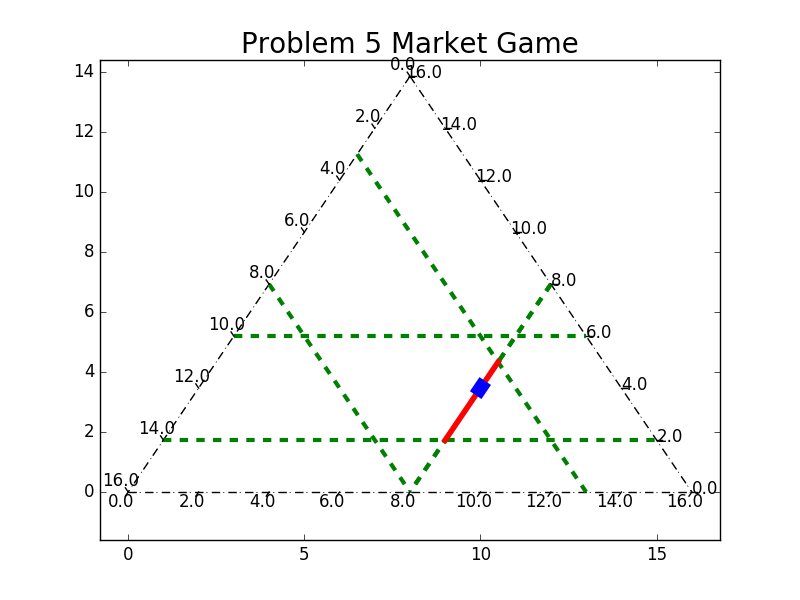
\includegraphics[width=.4\linewidth]{05_b}
      \caption{A graph of the core of the game on the 3-D simplex (solid red line) and the competitve solution (blue point) for the game.}
      \label{fig:05_b}
    \end{figure}
    
    %
    % Python code for plot
    %
    % import ternary

    % FONT_SIZE = 20
    % LINE_ARGS = {'linewidth': 3.0, 'linestyle': '--', 'color': 'green'}
    % CORE_ARGS = {'linewidth': 4.0, 'linestyle': 'solid', 'color': 'red'}

    % #
    % # Original
    % #
    % scale = 16
    % figure, tax = ternary.figure(scale=scale)

    % # Draw Boundary and Gridlines
    % tax.boundary(linewidth=1.0, linestyle='--')
    % tax.gridlines(color="black", multiple=scale / 4)

    % # Set Axis labels and Title
    % tax.set_title("Problem 5 Market Game", fontsize=FONT_SIZE)


    % tax.left_parallel_line(2, **LINE_ARGS)   # x1
    % tax.horizontal_line(3, **LINE_ARGS)      # x2
    % tax.right_parallel_line(8, **LINE_ARGS)  # x3
    % tax.right_parallel_line(8, **LINE_ARGS)
    % tax.horizontal_line(8, **LINE_ARGS)
    % tax.left_parallel_line(6, **LINE_ARGS)

    % tax.line(
    %     (8, 5, 3),  # not a solution, tweak to make the graph work
    %     (8, 2, 8),
    %     **CORE_ARGS)

    % tax.line((8, 4.05, 6), (8, 3.95, 6), color='blue', linewidth=10.0, linestyle='solid')

    % tax.ticks(axis='lbr', multiple=2.0, linewidth=1.0)

    % tax.show()




    %
    \item Verify that the vector $\Pi = (4, 2)$ is a price equilibrium vector for this game, by showing optimal consumptions (given $\Pi$) constitute an $N$-allocation. \\

    \textit{Solution}: \\
    To determine the lower bounds of allowable price vectors, we can examine the optimal allocations:
    \begin{align*}
    (w_{1}^{*}, w_{2}^{*}) &= \argmax u^{1}(w_{1}, w_{2}) - \Pi * (w_{1} - a^{1}_{1}, w_{2} - a^{1}_{2}) \\
                           &= \argmax 2w_{1} + 2w_{2} - \Pi_{1} * (w_{1} - 1) - \Pi_{2}(w_{2} - 0) \\
                           &= \argmax w_{1}(2 - \Pi_{1}) + w_{2}(2 - \Pi_{2}) + \Pi_{1} \\
                           &\implies \Pi_{1} \ge 2,\, \Pi_{2} \ge 2
    \end{align*}
    \begin{align*}
    (y_{1}^{*}, y_{2}^{*}) &= \argmax u^{2}(y_{1}, y_{2}) - \Pi * (y_{1} - a^{2}_{1}, y_{2} - a^{2}_{2}) \\
                           &= \argmax 4y_{1} + y_{2} - \Pi_{1} * (y_{1} - 0) - \Pi_{2}(y_{2} - 3) \\
                           &= \argmax y_{1}(4 - \Pi_{1}) + y_{2}(1 - \Pi_{2}) + 3\Pi_{2} \\
                           &\implies \Pi_{1} \ge 4,\, \Pi_{2} \ge 1
    \end{align*}
    \begin{align*}
    (z_{1}^{*}, z_{2}^{*}) &= \argmax u^{3}(z_{1}, z_{2}) - \Pi * (z_{1} - a^{3}_{1}, z_{2} - a^{3}_{2}) \\
                           &= \argmax 4\sqrt{z_{1}} + 4\sqrt{z_{2}} - \Pi_{1} * (z_{1} - 1) - \Pi_{2}(z_{2} - 1) \\
                           &= \argmax \sqrt{z_{1}}(4 - \Pi_{1}\sqrt{z_{1}}) + \sqrt{z_{2}}(4 - \Pi_{1}\sqrt{z_{2}}) + \Pi_{1} + \Pi_{2} \\
                           & \text{(assuming that we allocate the maximum available goods } (2, 4) \text{ to z)} \\
                           &\implies \Pi_{1} \ge \frac{4}{\sqrt{2}},\, \Pi_{2} \ge 2
    \end{align*}
    Taken together, this $\implies \Pi_{1} \ge 4,\, \Pi_{2} \ge 2$. (We take the most restrictive lower bound to ensure that no player is motivated to demand an infinite amount of any good)

    To determine the upper bounds of possible price vectors, we can examine the utility functions to see at what price a good would be profitable to purchase:
    \begin{align*}
    u^{1}(w_{1}, w_{2}) &= 2w_{1} + 2w_{2} \\
                        &\implies \Pi_{1}w_{1} \le 2w_{1} \implies \Pi_{1} \le 2 \\
                        &\implies \Pi_{2}w_{2} \le 2w_{2} \implies \Pi_{2} \le 2 \\\\
    u^{2}(y_{1}, y_{2}) &= 4y_{1} + y_{2} \\
                        &\implies \Pi_{1}y_{1} \le 4y_{1} \implies \Pi_{1} \le 4 \\
                        &\implies \Pi_{2}y_{2} \le  y_{2} \implies \Pi_{2} \le 1 \\\\
    u^{3}(z_{1}, z_{2}) &= 4\sqrt{z_{1}} + 4\sqrt{z_{2}} \\
                        & \text{(assuming that we allocate the maximum available goods } (2, 4) \text{ to z)} \\
                        &\implies \Pi_{1}z_{1} \le 4\sqrt{z_{1}} \implies \Pi_{1} \le \frac{4}{\sqrt{z_{1}}} \implies \Pi_{1} \le \frac{4}{\sqrt{2}} \\
                        &\implies \Pi_{2}z_{2} \le 4\sqrt{z_{2}} \implies \Pi_{2} \le \frac{4}{\sqrt{z_{2}}} \implies \Pi_{2} \le 2
    \end{align*}
    Taken together, this $\implies \Pi_{1} \le 4,\, \Pi_{2} \le 2$. (We take the least restrictive upper bound to allow at least one person to purchase the goods and others to sell their goods for a good price)

    If $\Pi = (4, 2)$, then we have $4 \le \Pi_{1} = 4 \le 4$ and $2 \le \Pi_{2} = 2 \le 2$, thus $\Pi$ is an equilibrium vector.

    %
    \hfill\newline
    \item Find the competitive solution to the game which corresponds with $\Pi$. \\

    \textit{Solution}: \\
    \[ \vec{\beta} = (4, 6, 8) \]
    Using the optimal consumptions found when finding $V(N)$ and the price equilibrium vector from the previous exercise, we can compute a competitive solution $\vec{\beta}$:
    \begin{align*}
    \beta_{1} &= u^{1}(w_{1}^{*}, w_{2}^{*}) + \Pi    * (\vec{a}^{1} - \vec{w}^{*}) \\
              &= 2(0) + 2(3)                 + (4, 2) * ((1, 0)      - (0, 3)) \\
              &= 6                           + (4, 2) * (1, -3) \\
              &= 6                           + -2 \\
              &= 4 \\\\
    \beta_{2} &= u^{2}(y_{1}^{*}, y_{2}^{*}) + \Pi    * (\vec{a}^{2} - \vec{y}^{*}) \\
              &= 4(1) + (0)                  + (4, 2) * ((0, 3)      - (1, 0)) \\
              &= 4                           + (4, 2) * (-1, 3) \\
              &= 4                           + 2 \\
              &= 6 \\\\
    \beta_{3} &= u^{2}(z_{1}^{*}, z_{2}^{*}) + \Pi    * (\vec{a}^{3} - \vec{z}^{*}) \\
              &= 4\sqrt{(1)} + 4\sqrt{(1)}   + (4, 2) * ((1, 1)      - (1, 1)) \\
              &= 0           + 8             + (4, 2) * (0, 0) \\
              &= 8                           - 0 \\
              &= 8
    \end{align*}
    $\vec{\beta}$ is in the core of the game, so it should be acceptable.

    \end{enumerate}

\end{enumerate}
%
\end{document}
